\PassOptionsToPackage{unicode=true}{hyperref} % options for packages loaded elsewhere
\PassOptionsToPackage{hyphens}{url}
%
\documentclass[]{article}
\usepackage{lmodern}
\usepackage{amssymb,amsmath}
\usepackage{ifxetex,ifluatex}
\usepackage{fixltx2e} % provides \textsubscript
\ifnum 0\ifxetex 1\fi\ifluatex 1\fi=0 % if pdftex
  \usepackage[T1]{fontenc}
  \usepackage[utf8]{inputenc}
  \usepackage{textcomp} % provides euro and other symbols
\else % if luatex or xelatex
  \usepackage{unicode-math}
  \defaultfontfeatures{Ligatures=TeX,Scale=MatchLowercase}
\fi
% use upquote if available, for straight quotes in verbatim environments
\IfFileExists{upquote.sty}{\usepackage{upquote}}{}
% use microtype if available
\IfFileExists{microtype.sty}{%
\usepackage[]{microtype}
\UseMicrotypeSet[protrusion]{basicmath} % disable protrusion for tt fonts
}{}
\IfFileExists{parskip.sty}{%
\usepackage{parskip}
}{% else
\setlength{\parindent}{0pt}
\setlength{\parskip}{6pt plus 2pt minus 1pt}
}
\usepackage{hyperref}
\hypersetup{
            pdftitle={Topic 2: Exercise 1},
            pdfauthor={Daniel Alonso},
            pdfborder={0 0 0},
            breaklinks=true}
\urlstyle{same}  % don't use monospace font for urls
\usepackage[margin=1in]{geometry}
\usepackage{color}
\usepackage{fancyvrb}
\newcommand{\VerbBar}{|}
\newcommand{\VERB}{\Verb[commandchars=\\\{\}]}
\DefineVerbatimEnvironment{Highlighting}{Verbatim}{commandchars=\\\{\}}
% Add ',fontsize=\small' for more characters per line
\usepackage{framed}
\definecolor{shadecolor}{RGB}{248,248,248}
\newenvironment{Shaded}{\begin{snugshade}}{\end{snugshade}}
\newcommand{\AlertTok}[1]{\textcolor[rgb]{0.94,0.16,0.16}{#1}}
\newcommand{\AnnotationTok}[1]{\textcolor[rgb]{0.56,0.35,0.01}{\textbf{\textit{#1}}}}
\newcommand{\AttributeTok}[1]{\textcolor[rgb]{0.77,0.63,0.00}{#1}}
\newcommand{\BaseNTok}[1]{\textcolor[rgb]{0.00,0.00,0.81}{#1}}
\newcommand{\BuiltInTok}[1]{#1}
\newcommand{\CharTok}[1]{\textcolor[rgb]{0.31,0.60,0.02}{#1}}
\newcommand{\CommentTok}[1]{\textcolor[rgb]{0.56,0.35,0.01}{\textit{#1}}}
\newcommand{\CommentVarTok}[1]{\textcolor[rgb]{0.56,0.35,0.01}{\textbf{\textit{#1}}}}
\newcommand{\ConstantTok}[1]{\textcolor[rgb]{0.00,0.00,0.00}{#1}}
\newcommand{\ControlFlowTok}[1]{\textcolor[rgb]{0.13,0.29,0.53}{\textbf{#1}}}
\newcommand{\DataTypeTok}[1]{\textcolor[rgb]{0.13,0.29,0.53}{#1}}
\newcommand{\DecValTok}[1]{\textcolor[rgb]{0.00,0.00,0.81}{#1}}
\newcommand{\DocumentationTok}[1]{\textcolor[rgb]{0.56,0.35,0.01}{\textbf{\textit{#1}}}}
\newcommand{\ErrorTok}[1]{\textcolor[rgb]{0.64,0.00,0.00}{\textbf{#1}}}
\newcommand{\ExtensionTok}[1]{#1}
\newcommand{\FloatTok}[1]{\textcolor[rgb]{0.00,0.00,0.81}{#1}}
\newcommand{\FunctionTok}[1]{\textcolor[rgb]{0.00,0.00,0.00}{#1}}
\newcommand{\ImportTok}[1]{#1}
\newcommand{\InformationTok}[1]{\textcolor[rgb]{0.56,0.35,0.01}{\textbf{\textit{#1}}}}
\newcommand{\KeywordTok}[1]{\textcolor[rgb]{0.13,0.29,0.53}{\textbf{#1}}}
\newcommand{\NormalTok}[1]{#1}
\newcommand{\OperatorTok}[1]{\textcolor[rgb]{0.81,0.36,0.00}{\textbf{#1}}}
\newcommand{\OtherTok}[1]{\textcolor[rgb]{0.56,0.35,0.01}{#1}}
\newcommand{\PreprocessorTok}[1]{\textcolor[rgb]{0.56,0.35,0.01}{\textit{#1}}}
\newcommand{\RegionMarkerTok}[1]{#1}
\newcommand{\SpecialCharTok}[1]{\textcolor[rgb]{0.00,0.00,0.00}{#1}}
\newcommand{\SpecialStringTok}[1]{\textcolor[rgb]{0.31,0.60,0.02}{#1}}
\newcommand{\StringTok}[1]{\textcolor[rgb]{0.31,0.60,0.02}{#1}}
\newcommand{\VariableTok}[1]{\textcolor[rgb]{0.00,0.00,0.00}{#1}}
\newcommand{\VerbatimStringTok}[1]{\textcolor[rgb]{0.31,0.60,0.02}{#1}}
\newcommand{\WarningTok}[1]{\textcolor[rgb]{0.56,0.35,0.01}{\textbf{\textit{#1}}}}
\usepackage{graphicx,grffile}
\makeatletter
\def\maxwidth{\ifdim\Gin@nat@width>\linewidth\linewidth\else\Gin@nat@width\fi}
\def\maxheight{\ifdim\Gin@nat@height>\textheight\textheight\else\Gin@nat@height\fi}
\makeatother
% Scale images if necessary, so that they will not overflow the page
% margins by default, and it is still possible to overwrite the defaults
% using explicit options in \includegraphics[width, height, ...]{}
\setkeys{Gin}{width=\maxwidth,height=\maxheight,keepaspectratio}
\setlength{\emergencystretch}{3em}  % prevent overfull lines
\providecommand{\tightlist}{%
  \setlength{\itemsep}{0pt}\setlength{\parskip}{0pt}}
\setcounter{secnumdepth}{0}
% Redefines (sub)paragraphs to behave more like sections
\ifx\paragraph\undefined\else
\let\oldparagraph\paragraph
\renewcommand{\paragraph}[1]{\oldparagraph{#1}\mbox{}}
\fi
\ifx\subparagraph\undefined\else
\let\oldsubparagraph\subparagraph
\renewcommand{\subparagraph}[1]{\oldsubparagraph{#1}\mbox{}}
\fi

% set default figure placement to htbp
\makeatletter
\def\fps@figure{htbp}
\makeatother


\title{Topic 2: Exercise 1}
\author{Daniel Alonso}
\date{November 28th, 2020}

\begin{document}
\maketitle

\hypertarget{importing-libraries}{%
\paragraph{Importing libraries}\label{importing-libraries}}

\begin{Shaded}
\begin{Highlighting}[]
\KeywordTok{library}\NormalTok{(dplyr)}
\KeywordTok{library}\NormalTok{(Rcpp)}
\KeywordTok{library}\NormalTok{(JuliaCall)}
\end{Highlighting}
\end{Shaded}

\hypertarget{importing-data-as-described-by-exercise}{%
\paragraph{Importing data as described by
exercise}\label{importing-data-as-described-by-exercise}}

\begin{Shaded}
\begin{Highlighting}[]
\NormalTok{d <-}\StringTok{ }\KeywordTok{read.csv}\NormalTok{(}\StringTok{"../../datasets/Colleges.csv"}\NormalTok{)}
\end{Highlighting}
\end{Shaded}

\hypertarget{replacing-binary-variable-private-with-1-and-0}{%
\paragraph{Replacing binary variable Private with 1 and
0}\label{replacing-binary-variable-private-with-1-and-0}}

\begin{Shaded}
\begin{Highlighting}[]
\NormalTok{d}\OperatorTok{$}\NormalTok{Private <-}\StringTok{ }\KeywordTok{ifelse}\NormalTok{(d}\OperatorTok{$}\NormalTok{Private }\OperatorTok{==}\StringTok{ "Yes"}\NormalTok{, }\DecValTok{1}\NormalTok{, }\DecValTok{0}\NormalTok{)}
\end{Highlighting}
\end{Shaded}

\hypertarget{selecting-columns}{%
\paragraph{Selecting columns}\label{selecting-columns}}

\begin{Shaded}
\begin{Highlighting}[]
\NormalTok{data <-}\StringTok{ }\NormalTok{d }\OperatorTok\StringTok{ }\NormalTok{dplyr}\OperatorTok{::}\KeywordTok{select}\NormalTok{(}\StringTok{'Private'}\NormalTok{,}\StringTok{'Apps'}\NormalTok{,}\StringTok{'Accept'}\NormalTok{,}\StringTok{'Enroll'}\NormalTok{,}\StringTok{'F.Undergrad'}\NormalTok{)}
\end{Highlighting}
\end{Shaded}

\hypertarget{calculating-covariances}{%
\paragraph{Calculating covariances}\label{calculating-covariances}}

\begin{Shaded}
\begin{Highlighting}[]
\NormalTok{cov_matrix <-}\StringTok{ }\KeywordTok{cov}\NormalTok{(data)}
\NormalTok{cov_matrix}
\CommentTok{#>                   Private          Apps        Accept       Enroll  F.Undergrad}
\CommentTok{#> Private         0.1986559     -745.3552     -519.2042    -235.1942    -1330.764}
\CommentTok{#> Apps         -745.3552439 14978459.5301  8949859.8119 3045255.9876 15289702.474}
\CommentTok{#> Accept       -519.2042169  8949859.8119  6007959.6988 2076267.7627 10393582.435}
\CommentTok{#> Enroll       -235.1942393  3045255.9876  2076267.7627  863368.3923  4347529.884}
\CommentTok{#> F.Undergrad -1330.7637175 15289702.4742 10393582.4355 4347529.8841 23526579.326}
\end{Highlighting}
\end{Shaded}

\newpage

\hypertarget{calculating-correlations}{%
\paragraph{Calculating correlations}\label{calculating-correlations}}

\begin{Shaded}
\begin{Highlighting}[]
\NormalTok{corr_matrix <-}\StringTok{ }\KeywordTok{cov2cor}\NormalTok{(cov_matrix)}
\NormalTok{corr_matrix}
\CommentTok{#>                Private       Apps     Accept     Enroll F.Undergrad}
\CommentTok{#> Private      1.0000000 -0.4320947 -0.4752520 -0.5679078  -0.6155605}
\CommentTok{#> Apps        -0.4320947  1.0000000  0.9434506  0.8468221   0.8144906}
\CommentTok{#> Accept      -0.4752520  0.9434506  1.0000000  0.9116367   0.8742233}
\CommentTok{#> Enroll      -0.5679078  0.8468221  0.9116367  1.0000000   0.9646397}
\CommentTok{#> F.Undergrad -0.6155605  0.8144906  0.8742233  0.9646397   1.0000000}
\end{Highlighting}
\end{Shaded}

\hypertarget{experimenting-a-little-bit-with-the-private-variable}{%
\paragraph{Experimenting a little bit with the private
variable}\label{experimenting-a-little-bit-with-the-private-variable}}

Let's try changing the Yes to 0 and the No to 1 and checking the
covariances and correlations

\begin{Shaded}
\begin{Highlighting}[]
\NormalTok{d <-}\StringTok{ }\KeywordTok{read.csv}\NormalTok{(}\StringTok{"../../datasets/Colleges.csv"}\NormalTok{)}
\NormalTok{d}\OperatorTok{$}\NormalTok{Private <-}\StringTok{ }\KeywordTok{ifelse}\NormalTok{(d}\OperatorTok{$}\NormalTok{Private }\OperatorTok{==}\StringTok{ "Yes"}\NormalTok{, }\DecValTok{0}\NormalTok{, }\DecValTok{1}\NormalTok{)}
\NormalTok{data <-}\StringTok{ }\NormalTok{d }\OperatorTok\StringTok{ }\NormalTok{dplyr}\OperatorTok{::}\KeywordTok{select}\NormalTok{(}\StringTok{'Private'}\NormalTok{,}\StringTok{'Apps'}\NormalTok{,}\StringTok{'Accept'}\NormalTok{,}\StringTok{'Enroll'}\NormalTok{,}\StringTok{'F.Undergrad'}\NormalTok{)}
\end{Highlighting}
\end{Shaded}

\begin{Shaded}
\begin{Highlighting}[]
\NormalTok{cov_matrix <-}\StringTok{ }\KeywordTok{cov}\NormalTok{(data)}
\NormalTok{cov_matrix}
\CommentTok{#>                  Private         Apps       Accept       Enroll  F.Undergrad}
\CommentTok{#> Private        0.1986559 7.453552e+02 5.192042e+02     235.1942     1330.764}
\CommentTok{#> Apps         745.3552439 1.497846e+07 8.949860e+06 3045255.9876 15289702.474}
\CommentTok{#> Accept       519.2042169 8.949860e+06 6.007960e+06 2076267.7627 10393582.435}
\CommentTok{#> Enroll       235.1942393 3.045256e+06 2.076268e+06  863368.3923  4347529.884}
\CommentTok{#> F.Undergrad 1330.7637175 1.528970e+07 1.039358e+07 4347529.8841 23526579.326}
\NormalTok{corr_matrix <-}\StringTok{ }\KeywordTok{cov2cor}\NormalTok{(cov_matrix)}
\NormalTok{corr_matrix}
\CommentTok{#>               Private      Apps    Accept    Enroll F.Undergrad}
\CommentTok{#> Private     1.0000000 0.4320947 0.4752520 0.5679078   0.6155605}
\CommentTok{#> Apps        0.4320947 1.0000000 0.9434506 0.8468221   0.8144906}
\CommentTok{#> Accept      0.4752520 0.9434506 1.0000000 0.9116367   0.8742233}
\CommentTok{#> Enroll      0.5679078 0.8468221 0.9116367 1.0000000   0.9646397}
\CommentTok{#> F.Undergrad 0.6155605 0.8144906 0.8742233 0.9646397   1.0000000}
\end{Highlighting}
\end{Shaded}

We get the same numbers with reversed signs.

\newpage

\hypertarget{we-define-the-following-function-in-julia-to-help-our-understanding}{%
\subsubsection{We define the following function (in julia) to help our
understanding:}\label{we-define-the-following-function-in-julia-to-help-our-understanding}}

Takes the arguments:

\begin{verbatim}
- nrows: number of data to simulate (amount of rows)
- simulations: number of different times to simulate and average the results
- fixed_value_col: boolean parameter with true -> assigns a set of values between mins[1] and maxs[1] (other 2 parameters)
- reverse: boolean parameter that determines whether the 0s in the binary variable are assigned to the higher values or not
- sim_binaries: this would simulate a rolling proportion of binaries where iteration 1 has all zeros in the binary variable and iteration *nrows* has all 1s in the binary variable
- mins: array containing as first element the minimum value to use for corresponding values in the quantitative columns with 1s and 0s assuming the fixed_value_col parameter is set to false, if it's set to true then it'll be the minimum of the quantitative variable we are calculating the covariance or correlation vs the quantitative variable. the second element of the array represents the same minimum but for the 2nd array which will substitute the values of elements that are 1 or 0 depending on the user choice. (for example: if reverse=false, fixed_value_col=false, maxs=[10,10000] and mins=[1,100],  the values in the quantitative variable corresponding to 1s in the binary variable will, as the loop goes on, go from having minimum value 1 to minimum value 100 and with will go from having maximum value 10 to maximum value 10000, therefore assigning high values (between 100-10000) to elements in the quant.variable corresponding to 1 in the binary variable and keep lower values (between 1-10) for the ones corresponding to 0s in the binary variable)
- maxs: same as minimum but they're the maximums.
\end{verbatim}

Example of how the dataset changes for a run of the function with
parameters: nrows=5, simulations=1 and the rest of the parameters as
default:

\begin{figure}
\centering
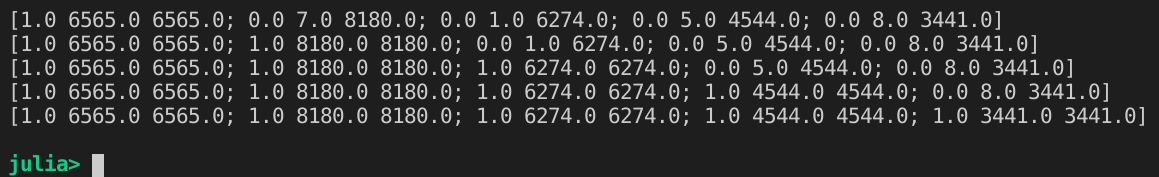
\includegraphics{julia_output.png}
\caption{Example of a simulated dataset with the function
simulation\_general in the Julia REPL}
\end{figure}

In Figure 1 we can see 5 iterations (as there's 5 simulated rows) using
the function, where the leftmost value of each row is a binary variable
(1 or 0), starting with (1,0,0,0,0) and ending with (1,1,1,1,1), and for
our quantitative variable (with which we will calculate cov/corr) we can
see the values go from a high value (copied from the 3rd column) and the
rest of values being small (6565,7,1,5,8) and ending with large values
(copied from column 3) being (6565, 8180, 6214, 4544, 3441).

\hypertarget{function-definition}{%
\subsubsection{Function definition}\label{function-definition}}

\begin{Shaded}
\begin{Highlighting}[]
\NormalTok{using Random}
\NormalTok{using Statistics}
\NormalTok{using Plots}
\NormalTok{gr()}
\CommentTok{#> Plots.GRBackend()}

\KeywordTok{function}\NormalTok{ simulation_general(nrows, simulations; fixed_value_col=false, reverse=false, sim_binaries=true, mins=[}\FloatTok{1}\NormalTok{,}\FloatTok{100}\NormalTok{], maxs=[}\FloatTok{10}\NormalTok{,}\FloatTok{10000}\NormalTok{]) }
    \CommentTok{# cov and corr matrixes}
\NormalTok{    covs = zeros(}\DataTypeTok{Float64}\NormalTok{, nrows, simulations)}
\NormalTok{    corr = zeros(}\DataTypeTok{Float64}\NormalTok{, nrows, simulations)}

    \CommentTok{# loop}
    \KeywordTok{for}\NormalTok{ s }\KeywordTok{in} \FloatTok{1}\NormalTok{:simulations}
\NormalTok{        pvtapps = zeros(}\DataTypeTok{Float64}\NormalTok{, nrows, }\FloatTok{3}\NormalTok{)}
        \KeywordTok{if}\NormalTok{ sim_binaries == false}
\NormalTok{            pvtapps[:,}\FloatTok{1}\NormalTok{] = rand(}\FloatTok{0}\NormalTok{:}\FloatTok{1}\NormalTok{, nrows)}
        \KeywordTok{end}

        \CommentTok{# random numbers column (quant variable)}
        \KeywordTok{if}\NormalTok{ fixed_value_col == true}
\NormalTok{            pvtapps[:,}\FloatTok{2}\NormalTok{] = rand(mins[}\FloatTok{1}\NormalTok{]:maxs[}\FloatTok{1}\NormalTok{],nrows)}
        \KeywordTok{else}
            \KeywordTok{if}\NormalTok{ reverse == false}
\NormalTok{                pvtapps[:,}\FloatTok{2}\NormalTok{] = rand(mins[}\FloatTok{1}\NormalTok{]:maxs[}\FloatTok{1}\NormalTok{],nrows)}
\NormalTok{                pvtapps[:,}\FloatTok{3}\NormalTok{] = rand(mins[}\FloatTok{2}\NormalTok{]:maxs[}\FloatTok{2}\NormalTok{],nrows)}
            \KeywordTok{else} 
\NormalTok{                pvtapps[:,}\FloatTok{2}\NormalTok{] = rand(mins[}\FloatTok{2}\NormalTok{]:maxs[}\FloatTok{2}\NormalTok{],nrows)}
\NormalTok{                pvtapps[:,}\FloatTok{3}\NormalTok{] = rand(mins[}\FloatTok{1}\NormalTok{]:maxs[}\FloatTok{1}\NormalTok{],nrows)}
            \KeywordTok{end}
        \KeywordTok{end}

        \CommentTok{# loop for changing values}
        \KeywordTok{for}\NormalTok{ i }\KeywordTok{in} \FloatTok{1}\NormalTok{:nrows}

            \KeywordTok{if}\NormalTok{ sim_binaries == true}
\NormalTok{                pvtapps[}\FloatTok{1}\NormalTok{:i,}\FloatTok{1}\NormalTok{] = ones(i)}
            \KeywordTok{end}

\NormalTok{            pvtapps[}\FloatTok{1}\NormalTok{:i,}\FloatTok{2}\NormalTok{] = pvtapps[}\FloatTok{1}\NormalTok{:i,}\FloatTok{3}\NormalTok{]}

            \CommentTok{# calculate corr and cov}
\NormalTok{            covs[i,s] = cov(pvtapps[:,}\FloatTok{1}\NormalTok{],pvtapps[:,}\FloatTok{2}\NormalTok{])}
\NormalTok{            corr[i,s] = cor(pvtapps[:,}\FloatTok{1}\NormalTok{],pvtapps[:,}\FloatTok{2}\NormalTok{])}
        \KeywordTok{end}
    \KeywordTok{end}

    \CommentTok{# results}
\NormalTok{    covsrows = zeros(}\DataTypeTok{Float64}\NormalTok{, nrows)}
\NormalTok{    corrrows = zeros(}\DataTypeTok{Float64}\NormalTok{, nrows)}
    \KeywordTok{for}\NormalTok{ i }\KeywordTok{in} \FloatTok{1}\NormalTok{:nrows}
\NormalTok{        covsrows[i] = mean(covs[i,:])}
\NormalTok{        corrrows[i] = mean(corr[i,:])}
    \KeywordTok{end}

    \CommentTok{# return matrixes}
    \KeywordTok{return}\NormalTok{ covsrows, corrrows}
\KeywordTok{end}
\CommentTok{#> simulation_general (generic function with 1 method)}

\NormalTok{covsrows, corrrows = simulation_general(}\FloatTok{500}\NormalTok{,}\FloatTok{100}\NormalTok{, reverse=false, sim_binaries=true);}
\end{Highlighting}
\end{Shaded}

\newpage

\hypertarget{covariance-plot-with-500-data-points-and-100-simulations-averaged}{%
\paragraph{Covariance plot with 500 data points and 100 simulations
averaged}\label{covariance-plot-with-500-data-points-and-100-simulations-averaged}}

\begin{Shaded}
\begin{Highlighting}[]
\NormalTok{covsrows <-}\StringTok{ }\NormalTok{JuliaCall}\OperatorTok{::}\KeywordTok{julia_eval}\NormalTok{(}\StringTok{"covsrows"}\NormalTok{)}
\KeywordTok{plot}\NormalTok{(covsrows)}
\end{Highlighting}
\end{Shaded}

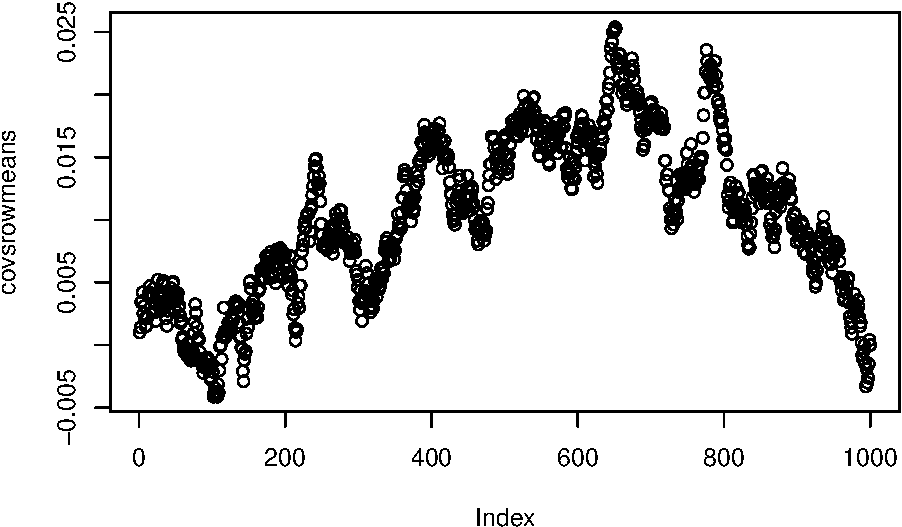
\includegraphics{./figures/unnamed-chunk-10-1.pdf}

We can see in our covariance plot

\hypertarget{correlation-plot-with-500-data-points-and-100-simulations-averaged}{%
\paragraph{Correlation plot with 500 data points and 100 simulations
averaged}\label{correlation-plot-with-500-data-points-and-100-simulations-averaged}}

\begin{Shaded}
\begin{Highlighting}[]
\NormalTok{corrrows <-}\StringTok{ }\NormalTok{JuliaCall}\OperatorTok{::}\KeywordTok{julia_eval}\NormalTok{(}\StringTok{"corrrows"}\NormalTok{)}
\KeywordTok{plot}\NormalTok{(corrrows)}
\end{Highlighting}
\end{Shaded}

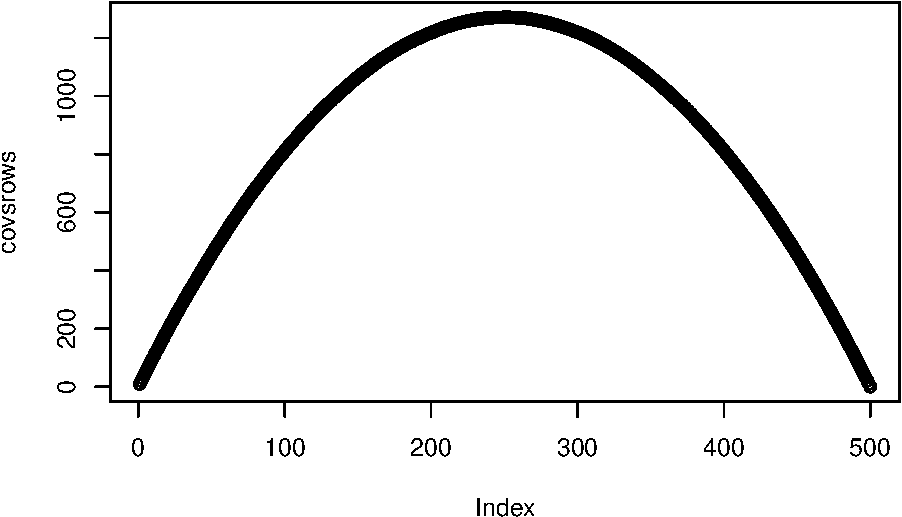
\includegraphics{./figures/unnamed-chunk-11-1.pdf}

\hypertarget{observations}{%
\section{OBSERVATIONS}\label{observations}}

Now let's play around changing the size of the values that correspond in
the quantitative variable to 1s or 0s in the binary column.

\hypertarget{what-information-does-the-sample-covariance-provide}{%
\subsection{What information does the sample covariance
provide?}\label{what-information-does-the-sample-covariance-provide}}

We know that because the Private variable (binary variable) has only 2
possible values, its covariance with other variables is always going to
be relatively small and will not provide much information.

\newpage

\hypertarget{what-information-does-the-sample-correlation-provide}{%
\subsection{What information does the sample correlation
provide?}\label{what-information-does-the-sample-correlation-provide}}

\end{document}
